\section{Introduction}

Machine learning and control theory are two foundational but disjoint communities.
Machine learning requires data to produce models, and control systems require models to provide stability, safety or other performance guarantees.
Machine learning is widely used for regression or classification, but thus far data-driven models have not been suitable for closed-loop control of physical plants.
The current challenge with data-driven approaches is to close the loop for real-time control and decision making.

For example, consider a multi-story building.
We ask the following questions.
\noindent (1) \textit{What should the optimal set-points be to curtail power consumption by 100 kW from 2-5pm tomorrow}?
Such actions are necessary for Demand Response (DR) when the price of electricity peaks due to high volatility.
For instance, in January 2014, the east coast electricity grid, managed by PJM, experienced an 86-fold increase in the price of electricity from \$31/MWh to \$2,680/MWh in a matter of 10 minutes.
\noindent (2) \textit{What are the optimal ways to cool or heat facilities in order to save energy and reduce carbon footprint?}
Automatic climate control while reducing the energy consumption is desirable under all circumstances. 
In large facilities and data centers this provides a huge financial incentive.

The first and foremost requirement for making such critical control decisions is to obtain the underlying control-oriented predictive model of the system.
With a reasonable forecast of the external disturbances, these models should predict the state of the system in the future and thus a predictive controller based on Model Predictive Control (MPC) can act preemptively to provide a desired behavior.
MPC has been proven to be very powerful for multivariable systems in the presence of input and output constraints, and forecast of the disturbances.
The caveat is that MPC requires a reasonably accurate mathematical model of the system.
Traditionally, for the building control, these mathematical models are built using first principles based on physics. 
The required effort for such model development and engineering, and the need for expert knowledge and periodic re-tuning of the model limit the use of physics-based models for MPC.
MPC has shown to be efficient supervisory control solution providing 17\% energy savings with better thermal comfort over rule-based control [1].
However, the key barrier is that it takes several months to capture accurate physics-based model of a medium to large-sized building.

There are three main reasons that make the modeling process hard for complex physical systems like buildings. 

\noindent \textbf{(1) Model capture} using only historical data is not suitable for control. Historical data, as large as it may be, does not capture the full model dynamics as the control set-points are based on rule-based strategies, thus lack in input excitation. Therefore, we need functional tests to excite the system with wide range of control inputs. However, in practice, functional tests are permitted only for a few hours in a month.

\noindent \textbf{(2) Change in model properties} over time - even if the model is identified once via an expensive route as in  \cite{Sturzenegger2016}, as the model changes with time, the system identification must be repeated to update the model. Thus, model adaptability or adaptive control is desirable for such systems. 

\noindent \textbf{(3) Model heterogeneity} further prohibits the use of model-based control. For example, unlike the automobile or the aircraft industry, each building is designed and used in a different way. Therefore, this modeling process must be repeated for every new building. 

Due to aforementioned reasons, the control strategies in such systems are often limited to fixed, sometimes ad-hoc, rules that are based on best practices. The key question now is: can we employ data-driven techniques to reduce the cost of modeling, and still exploit the benefits that MPC has to offer?
We therefore look for automatic data-driven approaches to control that are also adaptive and scalable.
We solve this problem by bridging the gap between Machine Learning and Predictive Control.

\subsection{Challenges in bridging machine learning and controls}
\label{SS:practical_challenges}

%The central idea is to obtain control-oriented models using machine learning or black-box modeling, and formulate the control problem in a way that receding horizon control (RHC) can still be applied and the optimization problem can be solved efficiently.

It is important to note that the standard machine learning regression used for prediction is fundamentally different from using machine learning for control synthesis. In the former, all the inputs to the model (also called regressors or features) are known, while in the latter some of the inputs that are the control variables must be optimized in real-time for desired performance. 
We next discuss the practical challenges in using machine learning algorithms for control.

\noindent \textbf{(1) Data quality:} Most of the historical data that are available from complex systems like buildings are based on some rule-based controllers. 
Therefore, the data may not be sufficient to explain the relationship between the inputs and the outputs. 
To obtain richer data with enough excitation in the inputs, new experiments must be done either by exciting the inputs randomly or by a procedure for optimal experiment design (OED) \cite{Emery1998,Fedorov2010}. 
This paper proposes a procedure for OED using Gaussian Processes (GP) to recommend control strategies.

\noindent \textbf{(2) Computational complexity:} Depending upon the learning algorithm, the output from a learned model is a non-linear, non-convex and sometimes non-differentiable (eg.~Random Forests \cite{Friedman2001}) function of the inputs with no closed-form expression. 
Using such models for control synthesis where some of the inputs must be optimized can lead to computationally intractable optimization. 
Our previous work uses an adaptation of Random Forests which overcomes this problem by separation of variables to derive a local linear input-output mapping at each time step \cite{JainCDC2017}.
This paper uses GPs for receding horizon control where the output mean and variance are analytical functions of the inputs, albeit non-convex.

\noindent \textbf{(3) Performance guarantees and robustness:} A desired characteristic for closed-loop control is to provide performance guarantees. 
This becomes hard when a black-box is used to replace a physical model. 
However, it is possible to provide probabilistic guarantees with a learning algorithm based on Gaussian Processes. 
GPs allow us to define chance constraints or account for model uncertainty in the cost while solving the optimization problem. This helps bound the performance errors with high confidence. 
Handling disturbance uncertainties or robustness to sensor failures in this framework is part of our on-going work and is thus excluded from this paper.

\noindent \textbf{(4) Model adaptability:} It is often the case that the model properties change with time, % (with seasons, for example),
and thus, the learned model must also be updated when required. 
The traditional mode of system identification, done repeatedly, can be time and cost prohibitive, especially in the case of buildings. 
In this paper, we show how GPs can be updated online to account for %seasonal
changes in the properties of the system.

%\noindent \textbf{(5) Interpretability of control decisions:} Besides the accuracy of synthesizing control strategies with machine learning in the loop, we are also interested in solutions that are interpretable and trustworthy. Thus, the DPC recommendations should have traceability so they can be verified to be stable and safe. This direction of research also forms part of our on-going work.

\subsection{Overcoming practical challenges}
To address these challenges, we can take two different approaches based on how machine learning is used to learn the models.

\noindent \textbf{(1) Mix of black-box and physics-based models:} In this approach, we use machine learning to learn only the dynamics of a sub-system or to model uncertainties in the dynamics. An example of former is in the use of machine learning for perception, and model-based control for low-level control in autonomous cars \cite{Urmson2008}. Examples on learning uncertainties in the models include \cite{Berkenkamp2015,Desaraju2016}.

\noindent \textbf{(2) Fully black-box models:} The full dynamical model can also be obtained using only machine learning algorithms. This deviates from the traditional notion of system identification where a physics-based structure is assumed to begin with. An example would be fully autonomous control using camera where control actions are mapped to raw image pixels \cite{Bojarski2016}. 
%The catch here is that, prior to learning, sufficiently large data could be generated by running the car in simulations.

For the application to building control in context of Demand Response, where there is a massive cost to physical modeling, this paper explores the latter route to bypass the modeling difficulties as summarized before. The data-driven approach allows to scale this methodology to multi-building campus and in general to many more applications like control of autonomous systems.

\subsection{Contributions}
\label{SS:contributions}
\begin{figure}[!t]
	\centering
	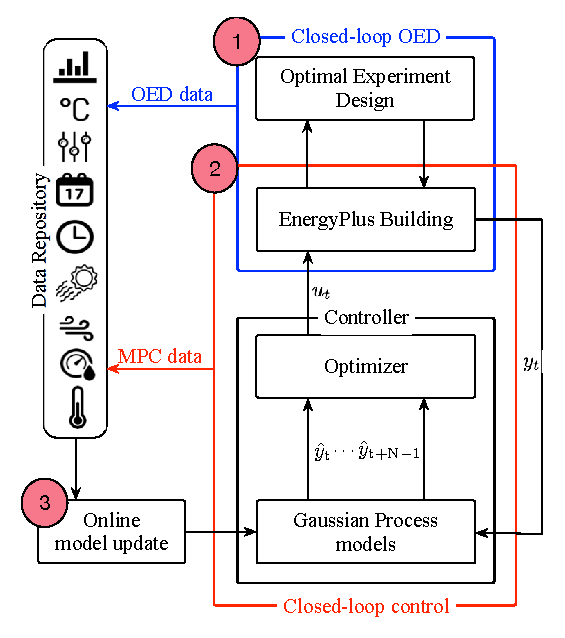
\includegraphics[width=0.7\linewidth]{figures/overview.eps}
	\caption{Paper contributions: (1) Optimal experiment design sequentially samples the inputs and applies to the system to generate training data, (2) Model Predictive Controller uses a Gaussian Process model learned on the OED data for receding horizon control, (3) the new data generated by controller is used to update the model online.}
	\captionsetup{justification=centering}
    \vspace{-11pt}
	\label{F:intro}
\end{figure}
This paper addresses the aforementioned practical challenges using fully black-box models based on Gaussian Processes.
In particular, this paper has the following contributions.

\noindent \textbf{(1) Optimal experiment design:} We develop a procedure for optimal experiment design with the dynamical system in a closed-loop by exploiting the variance in the predictions from a GP model. We show that under limited system availability and operation constraints, OED can provide faster learning rate than uniform random sampling or pseudo binary random sampling, reducing the duration of functional tests by upto \(50\%\).
	
\noindent \textbf{(2) Stochastic Model Predictive Control:} We show that the dynamical GP model can be used for real-time closed-loop finite horizon receding horizon control with probabilistic guarantees on constraint satisfaction. We again use the variance in the predictions from a GP model to make decisions where the model is most confident. In the case of Demand Response, we show that GP controller provides the necessary curtaiment with maximum \(1.7\% \) prediction error.
	
\noindent \textbf{(3) Online model update:} We propose an online method to update the GP model as new data are generated by running the GP-based controller in a closed-loop with the physical system.
Our method maximizes the information gain to select the best subset of data to update the model, thereby reducing the need for repetitive functional tests as systems properties change with time.

An overview of the organization is shown in Fig.~\ref{F:intro}.
We apply all three methods to large-scale buildings in EnergyPlus \cite{Deru2011}, a high fidelity building simulation software.
In the context of load curtailment for Demand Response, we apply OED to recommend control strategies to learn a model, fast and accurately. We show that MPC with GPs can provide the desired load curtailment with high confidence. After running the controller for a few weeks, we update the GP model with newly collected data, thus avoiding the need for a functional test in a new season.


\subsection{Related Work}
A broad range of data-driven modeling, assessment, and control methods for DR with buildings have been investigated in the literature.
Regression trees were used in our previous work \cite{JainCDC2017,JainACC2017,JainTCPS2018} to model and compute set-point schedules of buildings for DR.
Neural networks were used for MPC of a residential HVAC system in \cite{Afram2017} and Deep Reinforcement Learning for scheduling electrical devices in \cite{Mocanu2017}.
However, these methods require huge amount of data. 
On the other hand, GPs require only a few weeks of data, and our contributions put together, as described in Sec.~\ref{SS:contributions}, provide an end-to-end solution for learning and control.
GP models were investigated for forecasting long-term building energy consumption in \cite{nohetal13data}.
Simulation studies with EnergyPlus and regression models were used in \cite{yinetal16quantifying} to quantify the flexibility of buildings for DR using set-point change rules.
The authors in \cite{zhangetal15comparisons} compared four data-driven methods for building energy predictions and concluded that the Gaussian approaches were accurate and highly flexible, and the uncertainty measures could be helpful for certain applications involving risks.
In the experiment design literature, GPs were used for sensor placement to capture maximum information in \cite{Krause2008}, whereas our method, for the first time, sequentially recommends control strategies to generate more informative training data for the buildings.


%%% Local Variables:
%%% mode: latex
%%% TeX-master: "main"
%%% End:
